\section{User Interaction}\label{sec:interaction}
After initializing the flat mesh, we need to refine the model to final state through basic geometric constriant and user-selected constraints which are obtained from user interaction. Our system provides a set of operations to assist users construct the optimized model, such as automatically detecting merging vertexes and symmetric pair on given vertexes, and provide suggestions to allow users click the right option.

%Figure~\ref{fig:interface} illustrates two operations that the system provides, the first one is selecting points need to be merged by users and the second is select the right option from results by vertex merging detection.   

%\begin{figure}
%	\centering
%	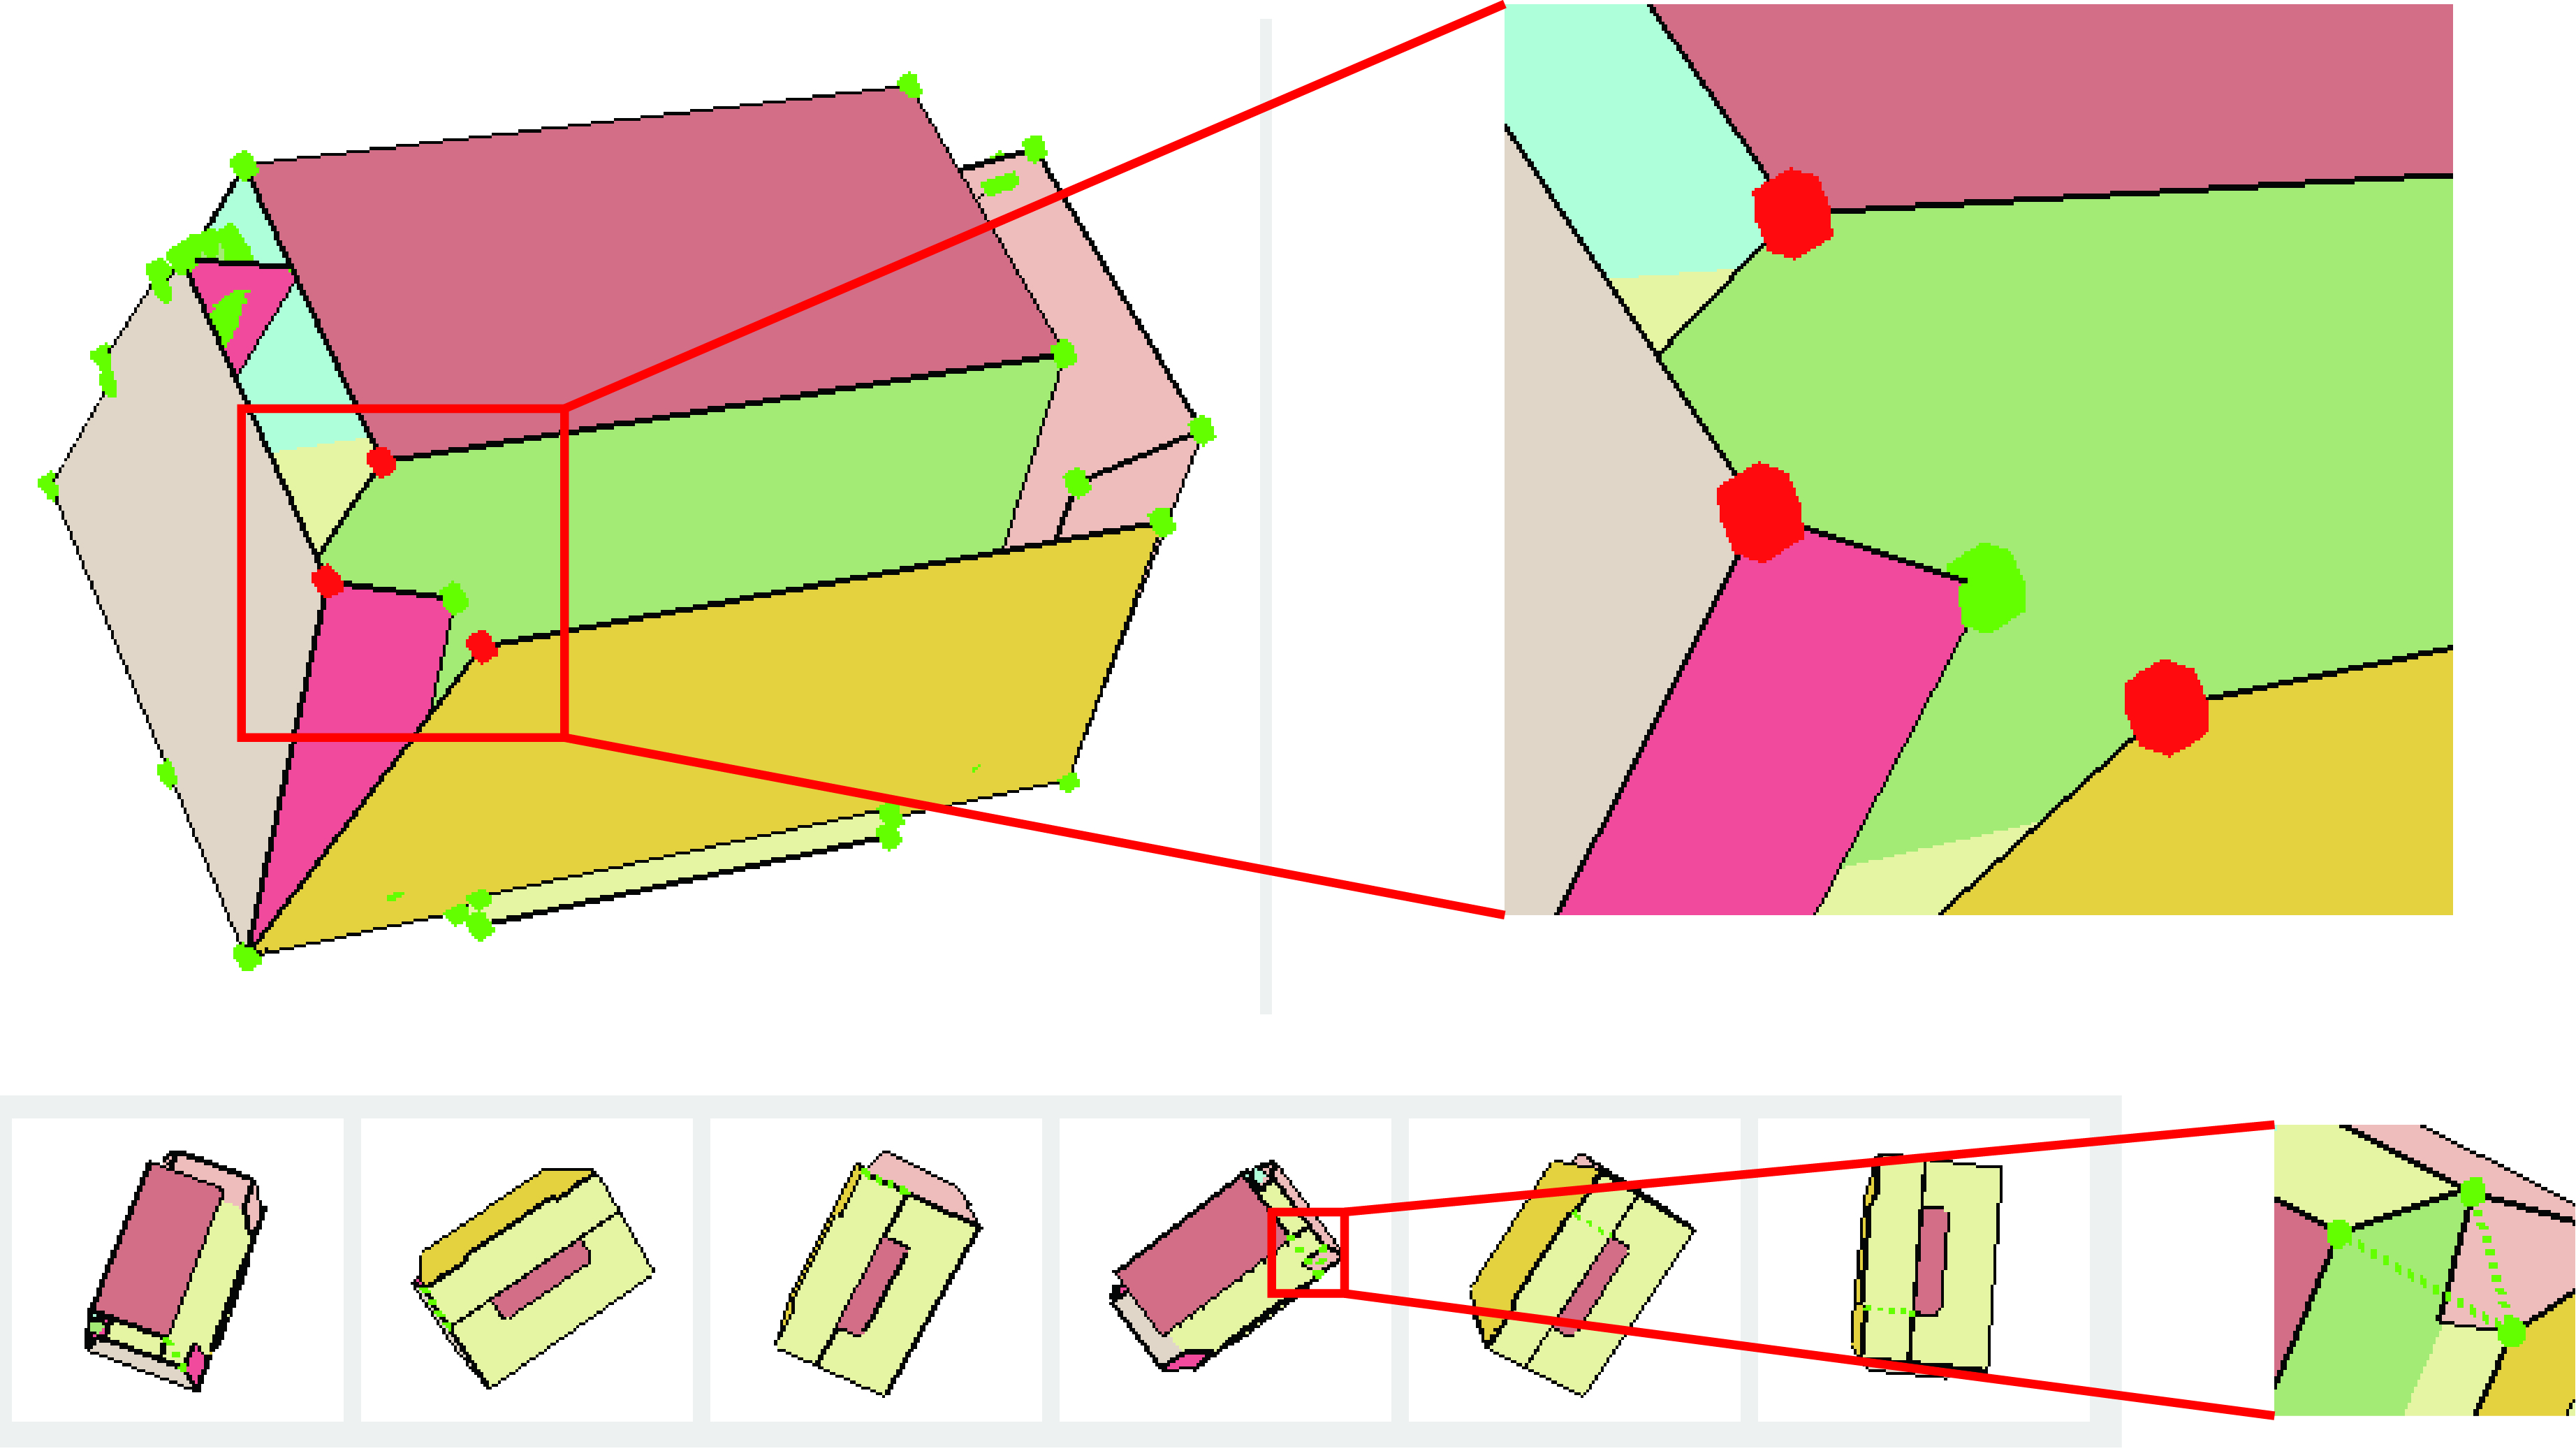
\includegraphics[width=0.9\textwidth]{images/UIdetail.jpg}
%	\caption{two operations that the system provides}
%	\label{fig:interface}
%\end{figure}

\subsection{Suggestive Interaction}

Our system automatically detects a group of potential shape constraints to form the final 3D model.
%
These guiding constraints are provided to the user for quickly selecting and manipulating the carton shape.
In our system, \cxj{two} types of shape refinement operations, vertex merging, and \cxj{shape symmetry}, are automatically detected.

%
%In order to assist users construct the final carton interactively, we also provide symmetry detection and merging points detection to improve the efficiency of constructing models .

\paragraph{Vertex Merging.} 
For irregular shapes which consist of non-rectangular faces or non-perpendicular adjacent faces, some vertexes are close to each other after the initialization step.
A practical carton model can be obtained by simply merging these nearby vertex together if their have coherent edge.
%
Any pair of vertexes $\mathbf{v}_a$, $\mathbf{v}_b$ that are in nonadjacent faces are detected as mergeable, if $|\mathbf{v}_a-\mathbf{v}_b|<\epsilon$, and there is an edge connecting to $\mathbf{v}_a$ having the equal length with one edge connecting to $\mathbf{v}_b$. 
%
\cxj{$\epsilon$ = ? in our experiments.}
More vertexes can be merged together, as shown in Figure~\ref{fig:suggestion}(a) by gradually adding one vertex $\mathbf{v}$ each time if $\mathbf{v}$ is mergeable with at least one vertex in current list. 
%Consider the initialization results can represent the ideal model partly, the disadjacent vertices that have one edge with same length can be regarded as targets that need to be located in the same place if their Euclidean distance is below a certain threshold.

\paragraph{Merging Propagation.} %{\color{blue}{focus on the symmetry property of vertexes.
Once the user makes a decision to merge a subset of vertexes $\mathbb{V}=\{\mathbf{v}_i\}_{i=1,\ldots,K}$ from automatic system suggestions, or manually selection, our system will detect if there exists another subset of vertexes $\vset_b$ symmetric to $\mathbb{V}$ and propagate the merging operation to $\vset_b$, as shown in Figure~\ref{fig:suggestion}(b). 
A subset $\mathbb{V}_b$ is symmetric to $\mathbb{V}_a$ if $|\vset_a|=|\vset_b|$, and there exists one-to-one correspondence between the vertexes in $\vset_a$ and $\vset_b$. 
Here, $|\vset|$ is the number of vertexes in a vertex subset $\vset$. 
Two vertexes $\vn_a$ and $\vn_b$ are defined as corresponding vertexes if they have the same number of edges and one-to-one correspondence can be found between the edge lengths. 


\comments{
	$\mathbf{v}_a$ and $\mathbf{v}_b$ are regarded as symmetric pair, if for each pair of $l_{ai} \in \{ l_{a1},l_{a2}...l_{am}\}$ and $l_{bi} \in \{ l_{b1},l_{b2}...l_{bn}\}$, $m = n$ and $|l_{ai}- l_{bi}|<\epsilon$ where $m$ is the number of $\mathbf{v}_a$'s ordered set of the incident edges' length $\{ l_{a1},l_{a2}...l_{am}\}$, and $n$ is the number of $\mathbf{v}_b$'s ordered set of the incident edges' length $\{ l_{b1},l_{b2}...l_{bn}\}$.
	
	When involving multiple vertexes, the searching criterion is based on symmetric vertex pair detection described above. The symmetric vertex set of selected vertexes $\{\mathbf{v}_1,\mathbf{v}_2,...,\mathbf{v}_{n-1}\}$ is $\{\hat{\mathbf{v}}_1,\hat{\mathbf{v}}_2,...,\hat{\mathbf{v}}_{n-1} \}$, the vertex set $\{\mathbf{v}_1,\mathbf{v}_2,...,\mathbf{v}_n\}$ has the symmetric vertex set $\{\hat{\mathbf{v}}_1,\hat{\mathbf{v}}_2,...,\hat{\mathbf{v}}_n \}$, if $||\mathbf{v}_n-\mathbf{v}_i| - |\hat{\mathbf{v}}_n-\hat{\mathbf{v}_i}||<\epsilon$, for $i = 1,....,n-1$.
}



\comments{Take Figure~\ref{fig:suggestion} (b) as an example, after users selecting vertexes circled in red, our system can automatically detect their symmetric set circled in blue. As an result, our system can detect these symmetry pairs to assist users improve efficiency.}

\paragraph{Face Pasting.} \cxj{ToBeDone}

\begin{figure}
	\centering
	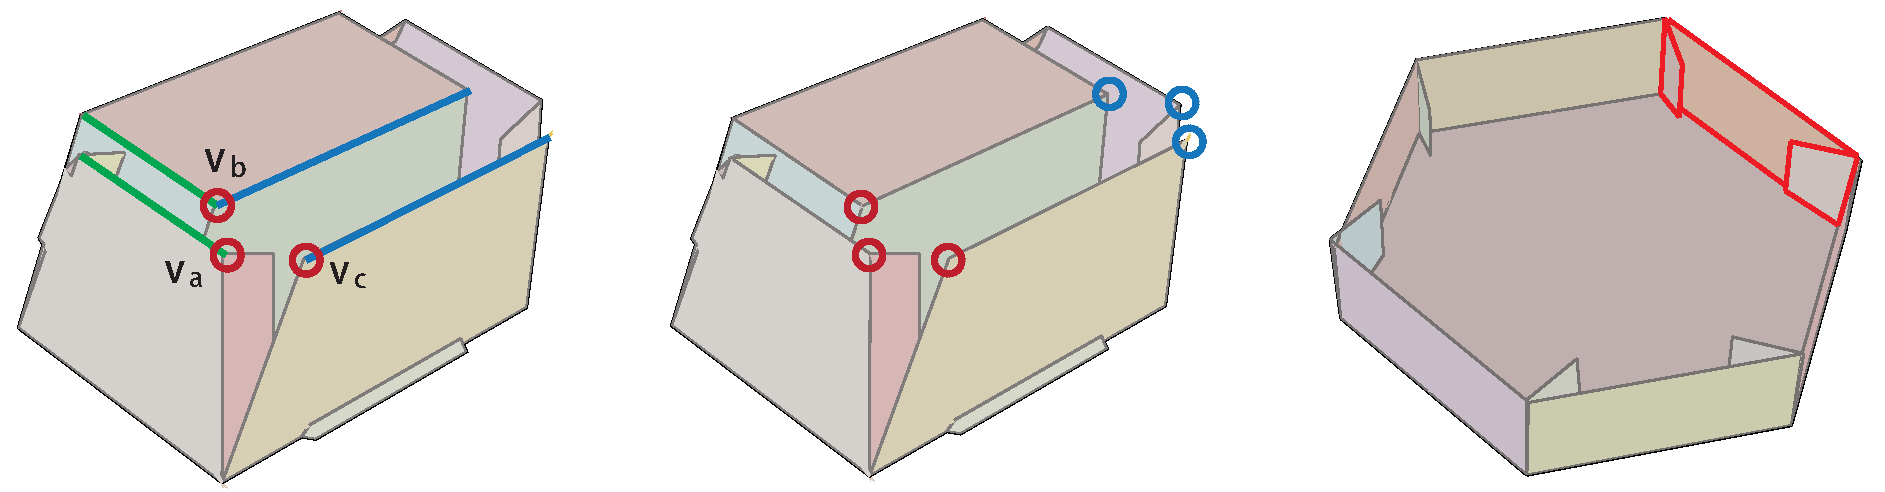
\includegraphics[width=0.9\textwidth]{images/suggestion}
	\caption{Vertex merging detection is well illustrated by (a), $\mathbf{v}_a$ and $\mathbf{v}_b$ may have the need to merge cause $|\mathbf{v}_a-\mathbf{v}_b|<\epsilon$, and one edge connecting to $\mathbf{v}_a$ marked as green has the same length with one edge connecting to $\mathbf{v}_b$ also marked as green. $\mathbf{v}_c$ can also be considered that need to merge with $\mathbf{v}_a$ and $\mathbf{v}_b$ as $|\mathbf{v}_c-\mathbf{v}_a(\mathbf{v}_b)|<\epsilon$ and one of incident edges of $\mathbf{v}_c$ marked as blue has the same length as $\mathbf{v}_a(\mathbf{v}_b)$'s also marked as blue. While users select three vertexes circled in red (b), our system can detect symmetric vertexes circled in blue automatically. \cxj{show more possible suggestions in this figure. Make sure the font in consistent with the caption}.\cxj{use subfigure?}}
	\label{fig:suggestion}
\end{figure}


\subsection{2D Layout Refinement from 3D Editing}


\cxj{Explain when modify the 3D model, how to change the 2D layout. }
{\color{blue}{In order to explore more design layouts, our system also allows users edit 3D models by dragging the edges into desired place, and enforce the geometric constraints similar to those described in Sec.~\ref{sec:refinement}. The edge length constraint and face rigidity are still the same, we expanded coplanarity to all the vertexes as they should lie on the same plane. The Irrelevant vertexes which exclude the two vertexes lie on the moving edge stay as close to their original location as well. Figure~\ref{fig:editing} shows one example of 3D editing.}}

\begin{figure}
	\centering
	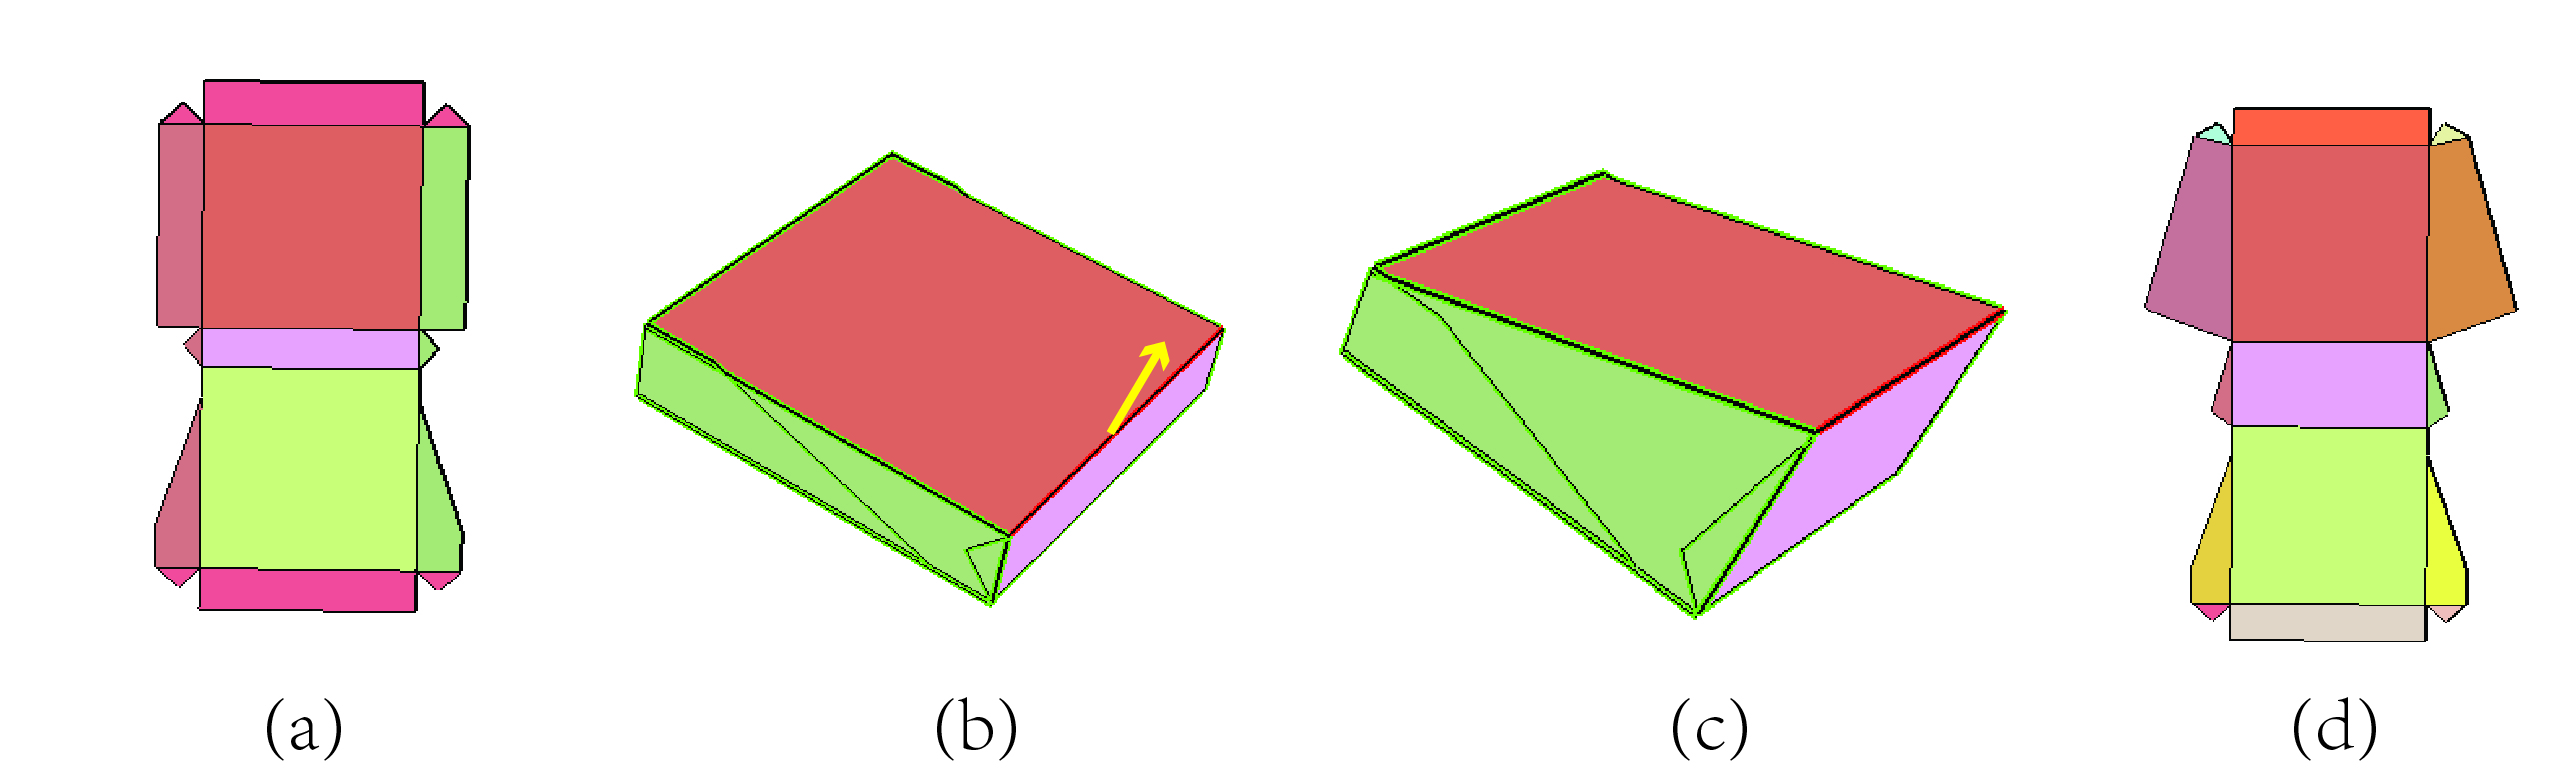
\includegraphics[width=0.6\textwidth]{images/editing}
	\caption{A standard cuboid carton (b) can be generated by the layout (a). Users are allowed to edit the shape of 3D model by dragging the edges, then the model will be deformed to a novel carton (c), by enforce the constrains to layout, our system can generate a deformable layout automatically as (d) shows.}
	\label{fig:editing}
\end{figure}